\documentclass[adobefonts, nocap]{ctexart}
\usepackage{amsmath}
\usepackage{amsfonts}
\usepackage{listings}
\usepackage{xcolor}
\usepackage{graphicx}
\usepackage{siunitx}
\usepackage{hyperref}
\hypersetup{
  colorlinks = true,
  linkcolor = blue,
  unicode = true
}
\lstset{
  language = C,
  basicstyle = \small\ttfamily,
  keywordstyle = \small\ttfamily\color{red},
  stringstyle = \color{gray},
  numbers = left,
  numberstyle = \small,
  numbersep = 5pt,
  frame = leftline,
  showstringspaces = false
}
\def\D{\mathrm{d}}
\begin{document}
  \title{计算机系统结构第四次作业}
  \author{李雨田\hspace{1em}2010012193\hspace{1em}计14}
  \maketitle
  \section*{1}
    对于LRU策略,不妨按照最近访问顺序,以链表的形式展示.从左到右分别是最近到最久访问过的缓存,每一行表示
    进行了其第一列指出的内存访问之后,缓存里的内容.得到缓存访问足迹,可算出
    命中率为$0.3$.

    \begin{center}
      \begin{tabular}{c||c|c|c|c}
        Ref & Head & Second & Third & Tail \\ \hline
        a (miss) & a & ~ & ~ & ~ \\
        b (miss) & b & a & ~ & ~ \\
        c (miss) & c & b & a & ~ \\
        a (hit) & a & c & b & ~ \\
        d (miss) & d & a & c & b \\
        e (miss) & e & d & a & c \\
        c (hit) & c & e & d & a \\
        d (hit) & d & c & e & a \\
        f (miss) & f & d & c & e \\
        a (miss) & a & f & d & c \\
      \end{tabular}
    \end{center}

    采用NRU策略可以得到以下结果.从左到右分别表示$4$个缓存行里面的内容.第一列表示的是内存访问,后四列表示
    进行内存访问之后,缓存里的内容.括号里数字表示NRU位.可以得到命中率同样为$0.3$.

    \begin{center}
      \begin{tabular}{c||c|c|c|c}
        Ref & Cache 0 & Cache 1 & Cache 2 & Cache 3 \\ \hline
        a (miss) & a (0) & (1) & (1) & (1) \\
        b (miss) & a (0) & b (0) & (1) & (1) \\
        c (miss) & a (0) & b (0) & c (0) & (1) \\
        a (hit) & a (0) & b (0) & c (0) & (1) \\
        d (miss) & a (0) & b (0) & c (0) & d (0) \\
        e (miss) & e (0) & b (1) & c (1) & d (1) \\
        c (hit) & e (0) & b (1) & c (0) & d (1) \\
        d (hit) & e (0) & b (1) & c (0) & d (0) \\
        f (miss) & e (0) & f (0) & c (0) & d (0) \\
        a (miss) & a (0) & f (1) & c (1) & d (1) \\
      \end{tabular}
    \end{center}

    采用$2$位SRRIP策略可以得到以下结果. $2$位RRPV可以表示$0$到$3$的数,即为括号中的数字.算得命中率为$0.4$,
    比之前两种方法都要高.

    \begin{center}
      \begin{tabular}{c||c|c|c|c}
        Ref & Cache 0 & Cache 1 & Cache 2 & Cache 3 \\ \hline
        a (miss) & a (2) & (3) & (3) & (3) \\
        b (miss) & a (2) & b (2) & (3) & (3) \\
        c (miss) & a (2) & b (2) & c (2) & (3) \\
        a (hit) & a (0) & b (2) & c (2) & (3) \\
        d (miss) & a (0) & b (2) & c (2) & d (2) \\
        e (miss) & a (1) & e (2) & c (3) & d (3) \\
        c (hit) & a (1) & e (2) & c (0) & d (3) \\
        d (hit) & a (1) & e (2) & c (0) & d (0) \\
        f (miss) & a (2) & f (2) & c (1) & d (1) \\
        a (hit) & a (0) & f (2) & c (1) & d (1) \\
      \end{tabular}
    \end{center}
  \section*{2}
    虽然题目没有指明,但这里可以认为采用的是写作废协议,而不是写更新协议.

    不难得到对于CPU请求的响应如下图所示.此处将发生替换的情况和未发生替换的情况一并画入同一状态转换图.和写回法不同的地方在于,
    发生写不命中的时候,均要回到状态I,而不是状态M.

    \begin{center}
      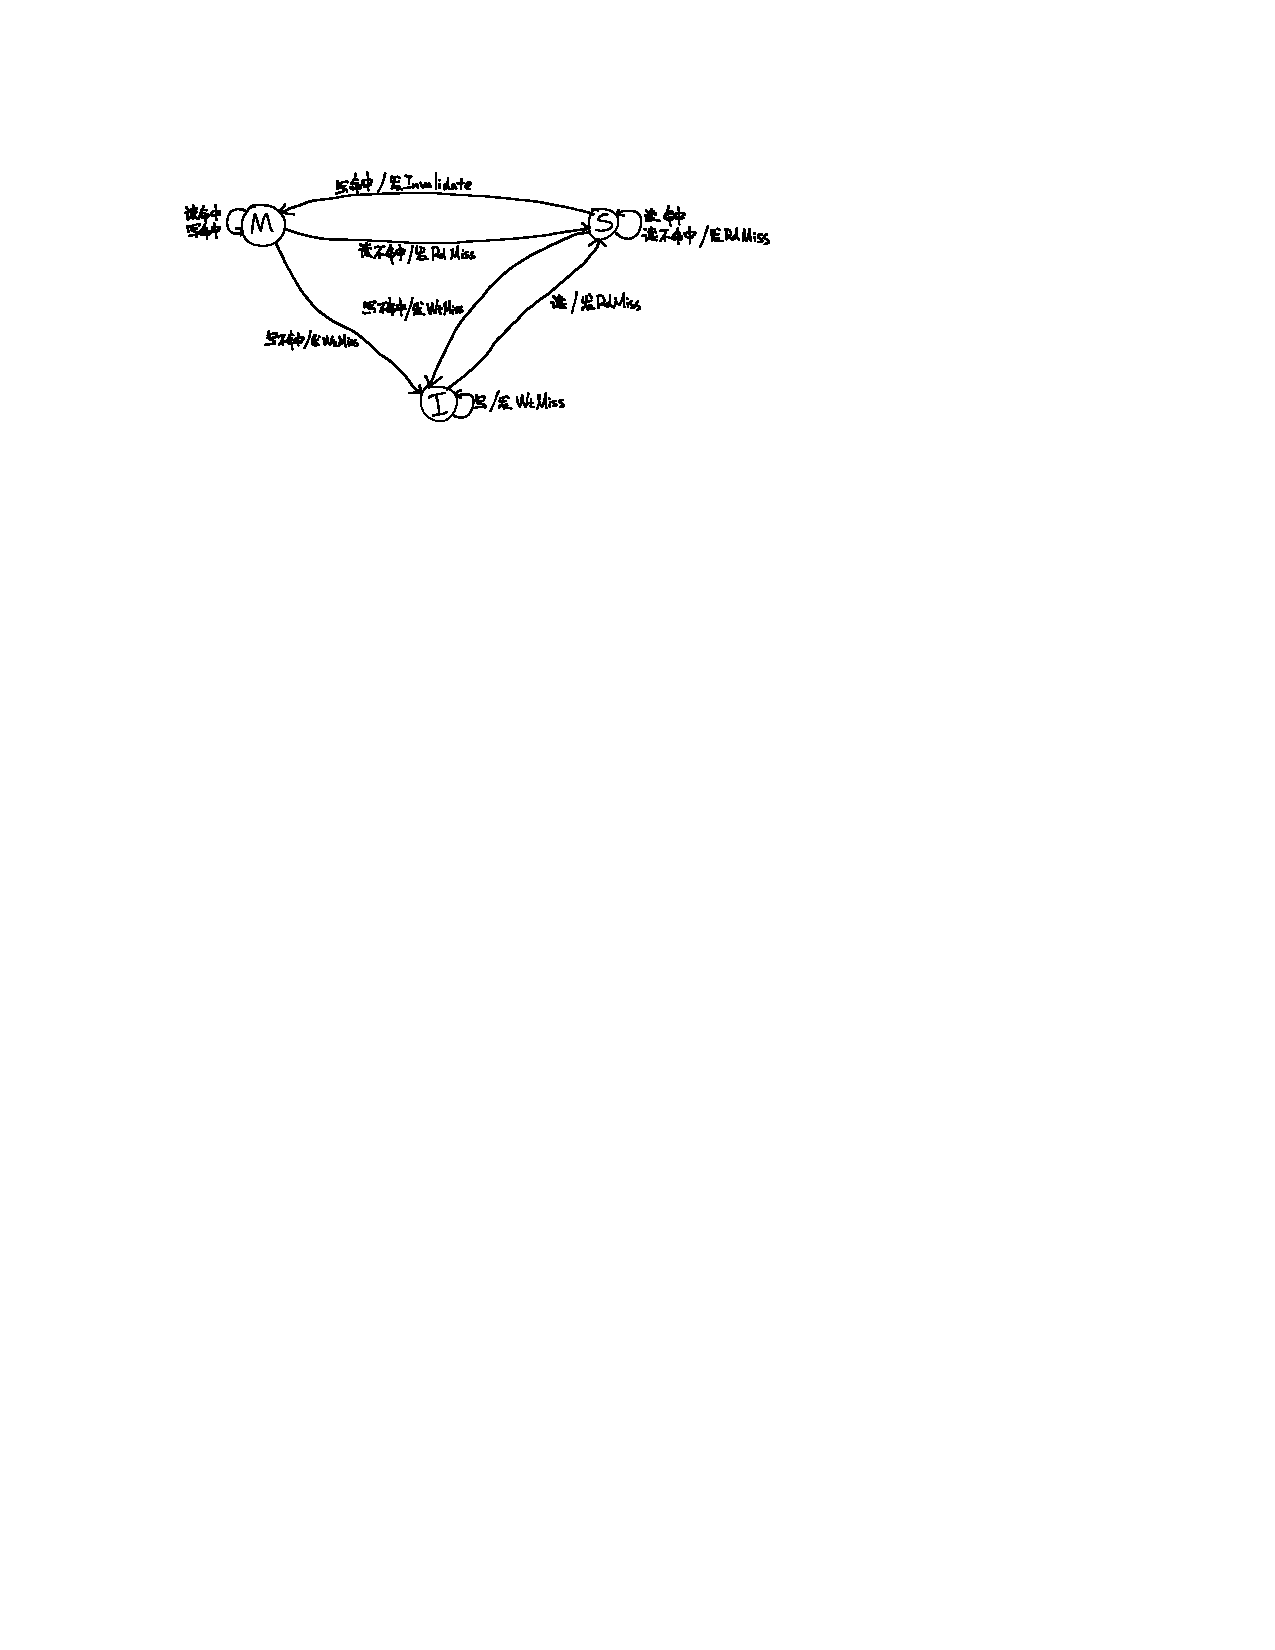
\includegraphics[width=10cm]{1-crop.pdf}
    \end{center}

    对于总线请求的响应如下图所示.和写回法基本一致.注意到M状态是不可能接受Invalidate请求的,因为当一份副本处于
    M状态时,其他副本不可能处于S状态.

    \begin{center}
      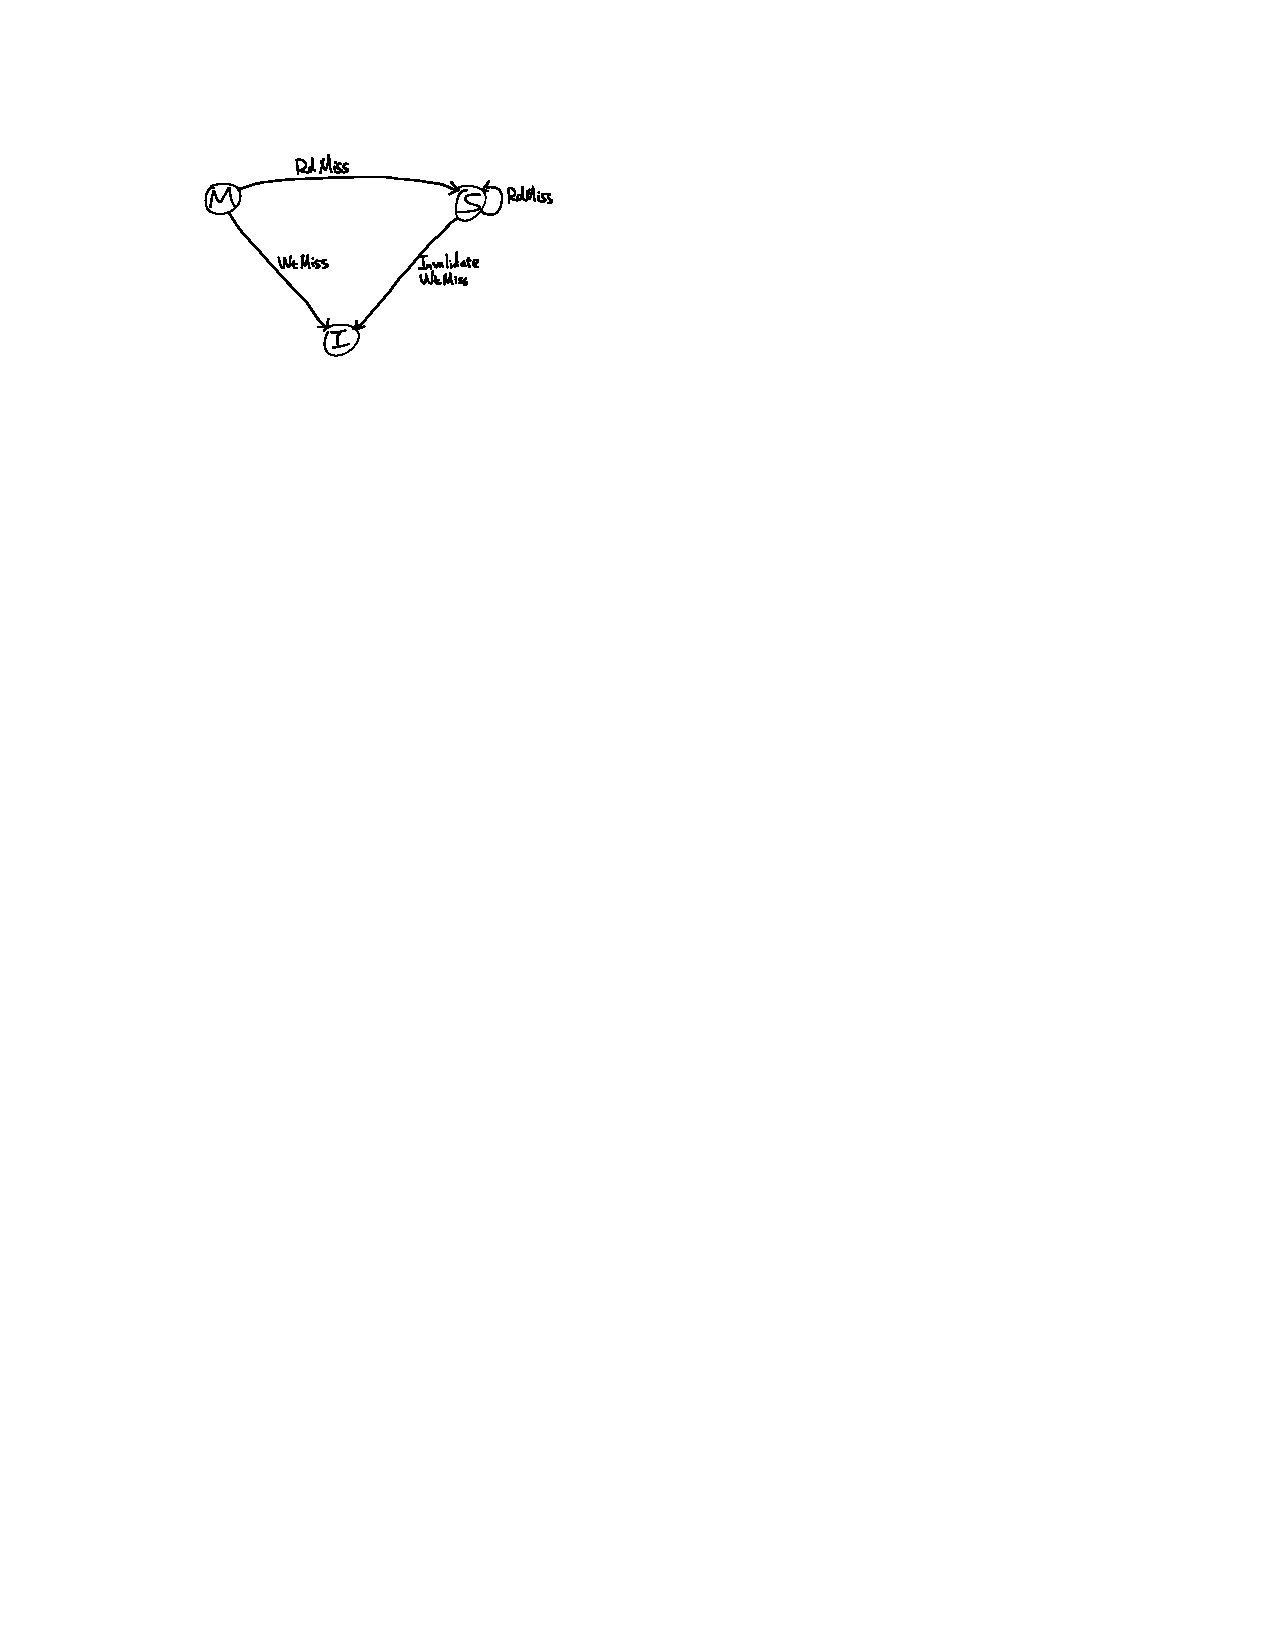
\includegraphics[width=10cm]{2-crop.pdf}
    \end{center}
  \section*{3}
    画出对于CPU请求的响应.此处相比之前多出的状态E即是Exclusive.此时虽然缓存没有写脏,但是只有一份副本.

    \begin{center}
      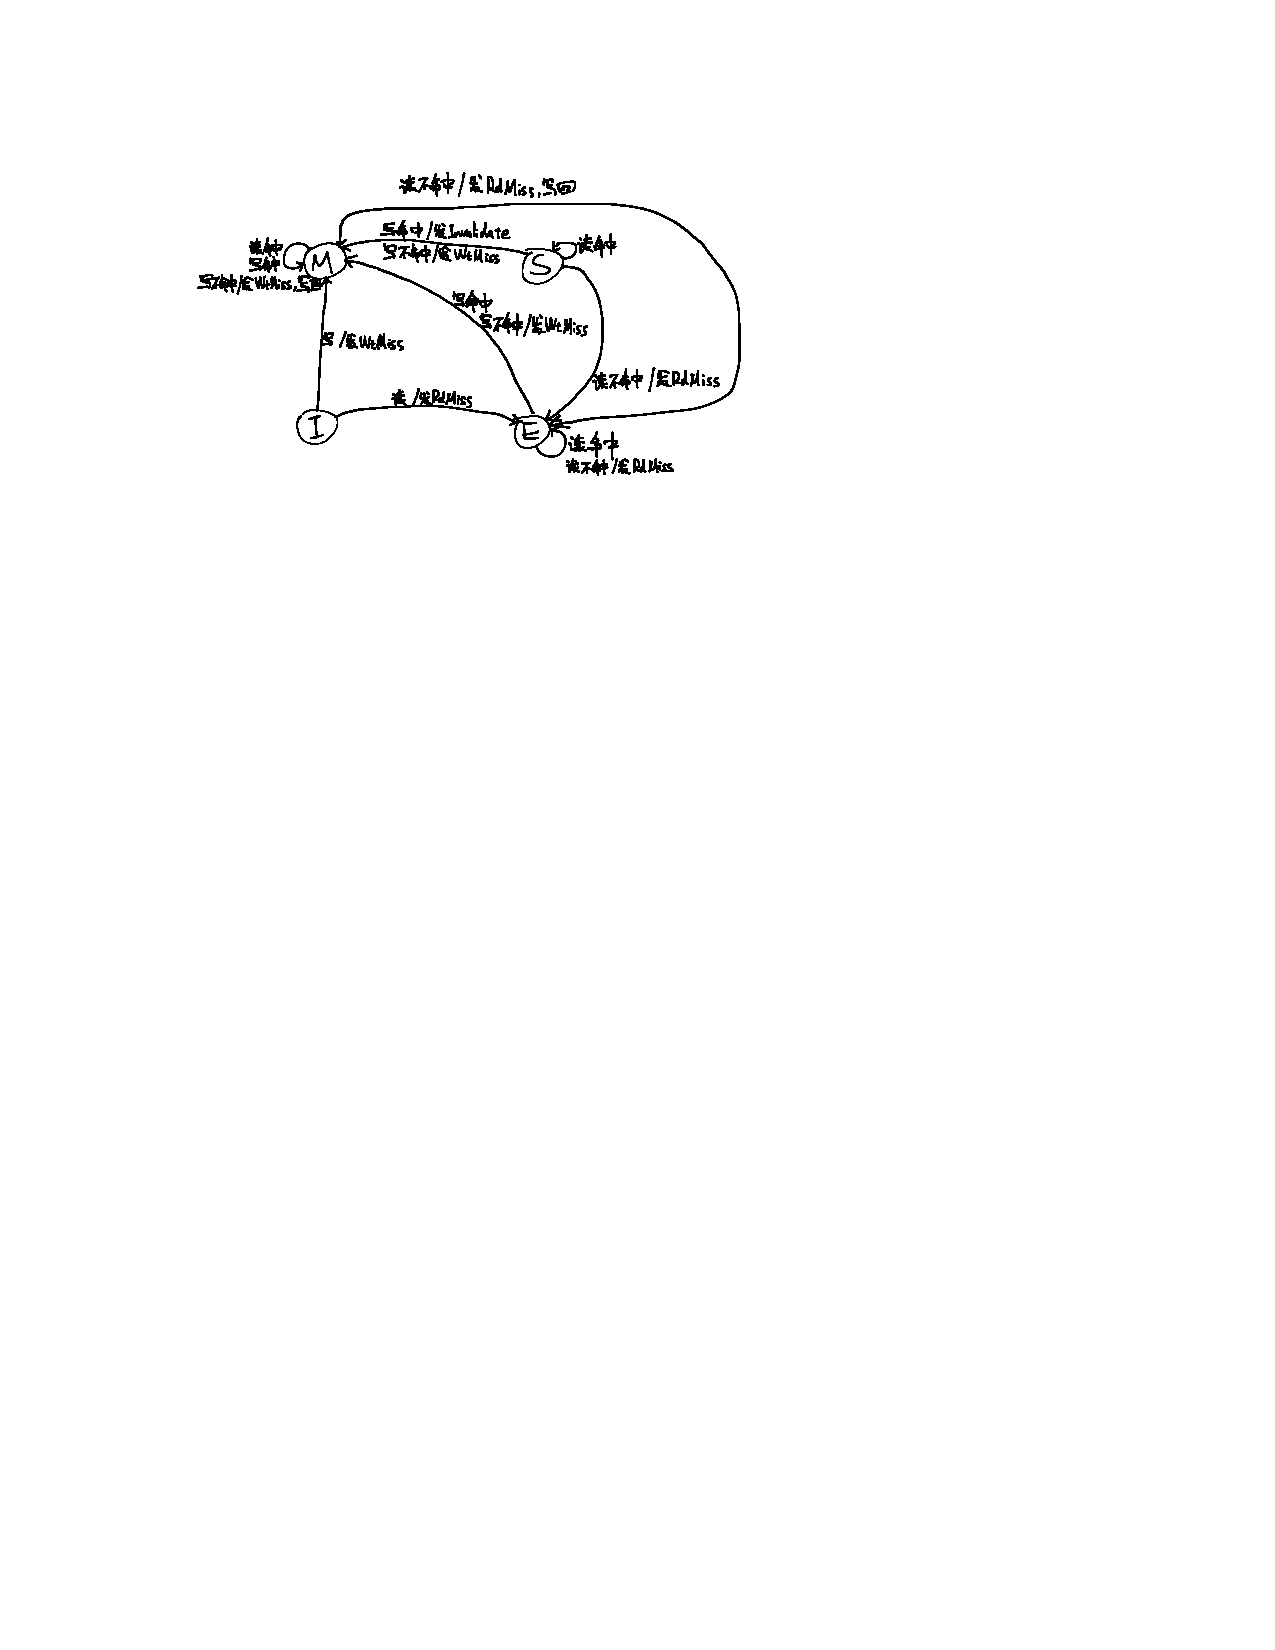
\includegraphics[width=10cm]{3-crop.pdf}
    \end{center}

    对于总线请求的响应如下图所示.注意到E状态下不会接收Invalidate请求,因为只有一份副本.如果其他CPU尝试
    写操作,则只会产生WtMiss请求.

    为了区分E状态和S状态,这里需要定义一个新的请求,称之为Share.即从内存读取到缓存中时,默认认为是处于E状态.
    但是读取的时候会产生RdMiss请求.如果其他副本接收到这个RdMiss请求,则会转换到S状态,并且发送Share请求.
    原始读入的缓存接收到这个Share请求,则会由E状态转换到S状态.简单说来,即是会检测其他缓存中是否有相同副本.
    如果有的话则转换到S状态,否则停留在E状态.

    \begin{center}
      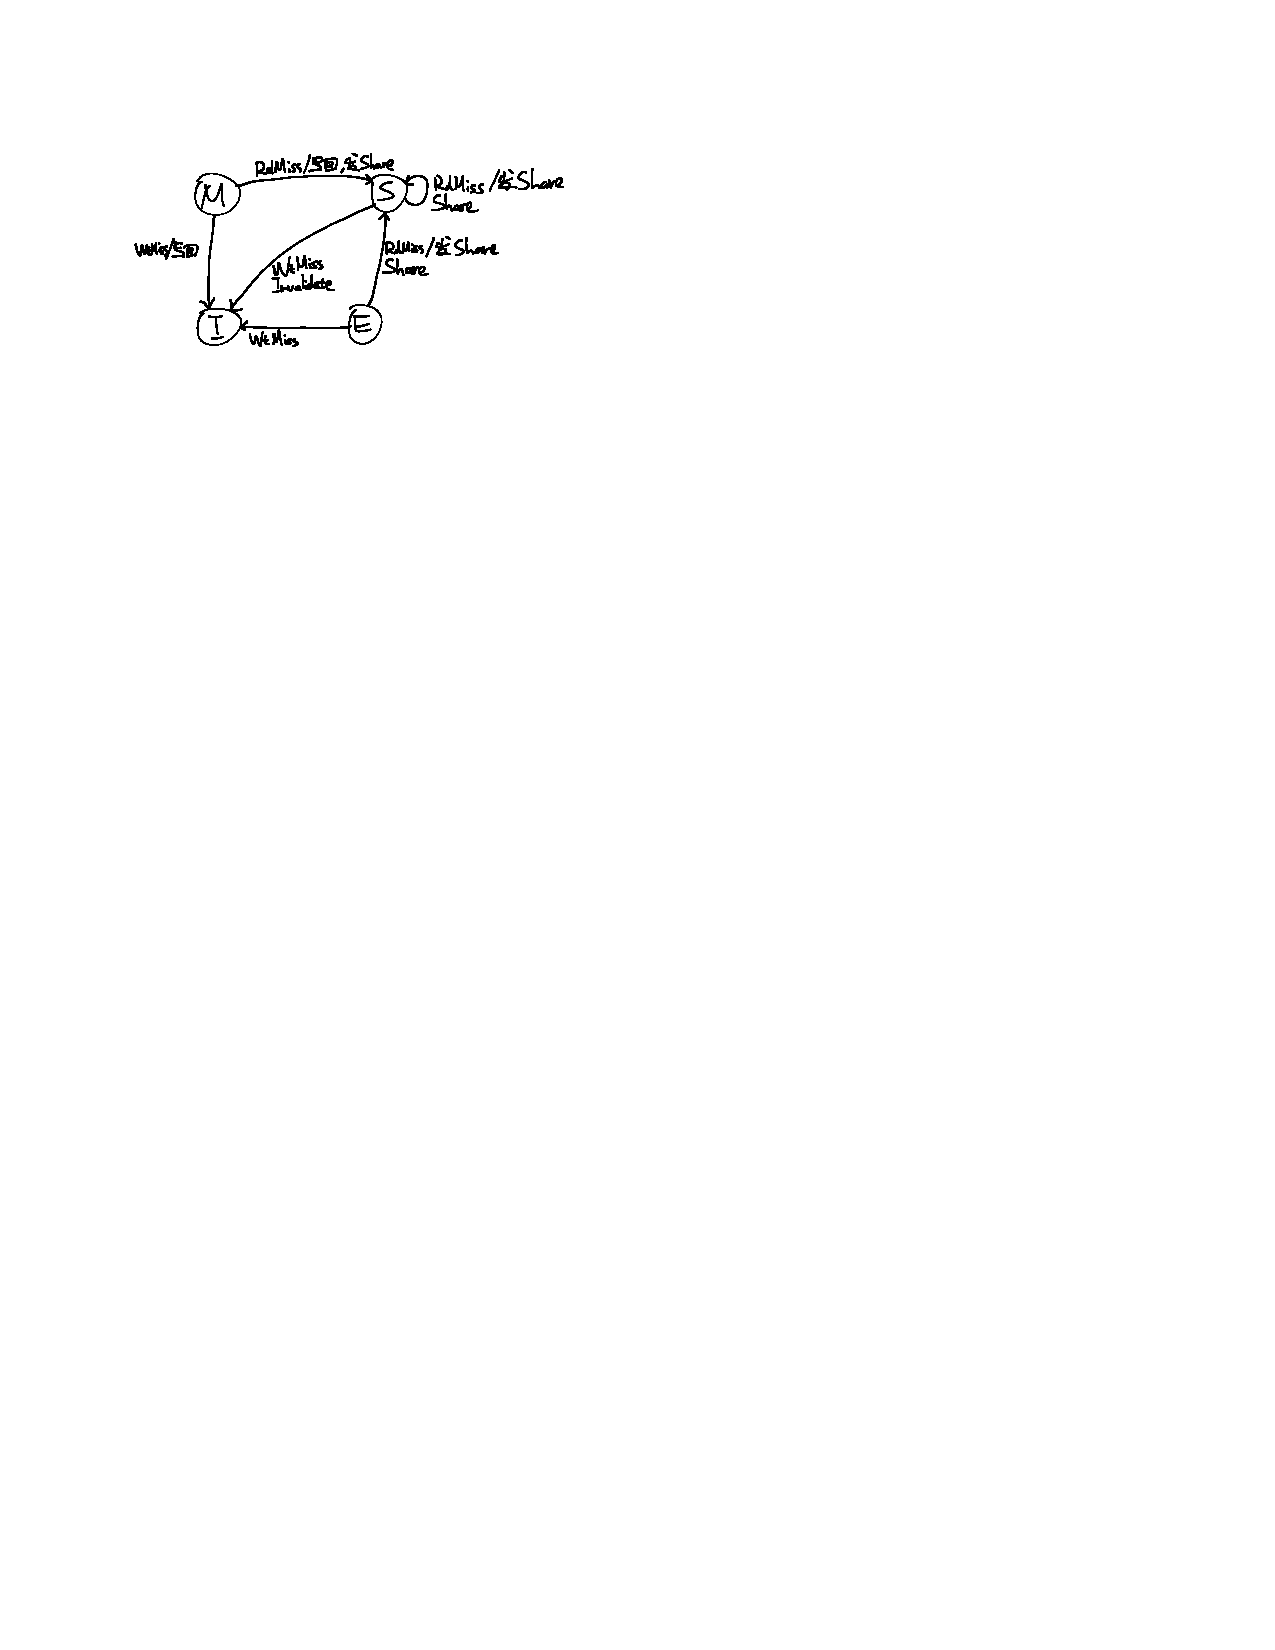
\includegraphics[width=10cm]{4-crop.pdf}
    \end{center}

    这种协议的优点在于,如果只有一份副本,那么第一次写脏的时候不用产生Invalidate请求.但是因为多一个状态
    会使得实现起来更加复杂,并且总线上可能会有更多的请求,所以最终不一定有性能上的提升.
\end{document}
